\documentclass[11pt]{article}

% template
\usepackage{if69d-template} % Modelo elaborado por Fernando Padilha

% pacotes
\usepackage[brazil]{babel}
\usepackage[utf8]{inputenc}
\usepackage[T1]{fontenc}
\usepackage{graphicx}
\usepackage{amsthm,amsfonts,amsmath}
\usepackage{newtxtext,newtxmath} % Times 11, como pede o modelo
\usepackage[font=footnotesize,
			labelfont=it,
			labelformat=simple]{subcaption}
\renewcommand\thesubfigure{(\alph{subfigure})}
\usepackage{booktabs}
\usepackage{url}
\graphicspath{{figuras/}}

% capa
\instituicao{Universidade Tecnológica Federal do Paraná -- UTFPR -- Campus Curitiba}
\departamento{Departamento Acadêmico de Eletrônica -- DAELN}
\curso{Curso de Engenharia de Computação}
\disciplina{IF69D e OPEET014 –- Processamento Digital de Imagens}
\semestre{2026.2}
\professor{Gustavo B. Borba e Humberto R. Gamba}

\titulo{Do alimento isolado ao prato: reconhecimento de alimentos com CNN e data augmentation}

\autor{Ana Luisa Girio}{2401070}
\date{11.2026}


\begin{document}

\maketitle

\section{Objetivo}

Explorar o banco de imagens bd\_porcoes\_alimentares~\cite{shiga} com redes neurais convolucionais (CNN), data augmentation e avaliação quantitativa. A tarefa escolhida foi analisar um prato: dada uma foto de cima, dizer quais dos 16 alimentos do banco estão presentes e onde. A dificuldade é que o banco só tem rótulos para fotos de um alimento sozinho, então o sistema aprende com alimentos isolados e precisa funcionar com eles misturados.

\section{Fundamentação Teórica}

\subsection{Segmentação clássica}

O espaço de cor CIELAB separa a luminância $L$ da cor $(a, b)$, e a distância euclidiana em $(a, b)$ aproxima a diferença de cor percebida, pouco afetada por sombras~\cite{gonzalez:18}. O prato branco é separado do fundo pelo método de Otsu~\cite{otsu:79}, que escolhe o limiar $t^*$ que maximiza a variância entre as duas classes de brilho (equação~\ref{eq:otsu}),

\begin{equation} \label{eq:otsu}
\sigma_B^2(t) = \omega_0(t)\,\omega_1(t)\,\big[\mu_0(t) - \mu_1(t)\big]^2, \qquad t^* = \arg\max_t \, \sigma_B^2(t)
\end{equation}

\noindent onde $\omega_0$ e $\omega_1$ são as proporções de pixels abaixo e acima de $t$, e $\mu_0$ e $\mu_1$ as suas médias.

A máscara é refinada por morfologia matemática~\cite{gonzalez:18}. Sendo $A$ a máscara binária e $B$ o elemento estruturante, a abertura remove objetos menores que $B$ e o fechamento preenche buracos menores que $B$ (equação~\ref{eq:morfo}),

\begin{equation} \label{eq:morfo}
A \circ B = (A \ominus B) \oplus B, \qquad A \bullet B = (A \oplus B) \ominus B
\end{equation}

\noindent onde $\ominus$ é a erosão e $\oplus$ a dilatação. Um pixel do prato é considerado comida se a distância de cor ao prato (equação~\ref{eq:dist}) ou a textura, medida pelo desvio padrão local de $L$, forem altas,

\begin{equation} \label{eq:dist}
d(x, y) = \sqrt{\big(a(x,y) - a_0\big)^2 + \big(b(x,y) - b_0\big)^2}
\end{equation}

\noindent onde $(a_0, b_0)$ é a mediana da cor dos pixels lisos do prato.

\subsection{CNN e data augmentation}

A ResNet~\cite{he:16} é uma CNN com conexões residuais. Partindo de pesos treinados na ImageNet~\cite{deng:09}, ela é ajustada ao novo problema (\textit{transfer learning}). Data augmentation gera variações das imagens de treino para reduzir o sobreajuste~\cite{shorten:19}. Uma variante mistura duas imagens num mesmo exemplo com rótulo proporcional à área de cada uma, como no CutMix~\cite{yun:19}; com esse rótulo suave $y$, a perda é a entropia cruzada da equação~\ref{eq:perda},

\begin{equation} \label{eq:perda}
\mathcal{L} = -\sum_k y_k \log p_k
\end{equation}

\noindent onde $p_k$ é a probabilidade da classe $k$ na saída softmax. Para verificar para onde a rede olha, usa-se o Grad-CAM~\cite{selvaraju:17}, que pondera os mapas de ativação da última camada convolucional pelo gradiente da classe.

\subsection{Métricas}

Cada foto tem um conjunto verdadeiro de alimentos $V$ e um conjunto previsto $P$. Por classe calculam-se a precisão $\mathrm{Prec} = \mathrm{VP}/(\mathrm{VP}+\mathrm{FP})$, o recall $\mathrm{Rec} = \mathrm{VP}/(\mathrm{VP}+\mathrm{FN})$ e o F1 (equação~\ref{eq:f1}), com média macro (mesmo peso para todas as classes) ou micro. Por foto, usa-se o índice de Jaccard (equação~\ref{eq:f1}); na segmentação, a mesma razão calculada em pixels é o IoU. Como as fotos foram tiradas em rajadas do mesmo prato, os intervalos de confiança são obtidos por bootstrap sobre pratos~\cite{efron:93}.

\begin{equation} \label{eq:f1}
F_1 = \frac{2\,\mathrm{Prec}\cdot\mathrm{Rec}}{\mathrm{Prec}+\mathrm{Rec}}, \qquad J(V, P) = \frac{|V \cap P|}{|V \cup P|}
\end{equation}

\section{Implementação}

O sistema foi implementado em Python com OpenCV e PyTorch. A Figura~\ref{fig:blocos} mostra o diagrama em blocos do treino e da análise de um prato.

\begin{figure}[!htb]
	\centering
	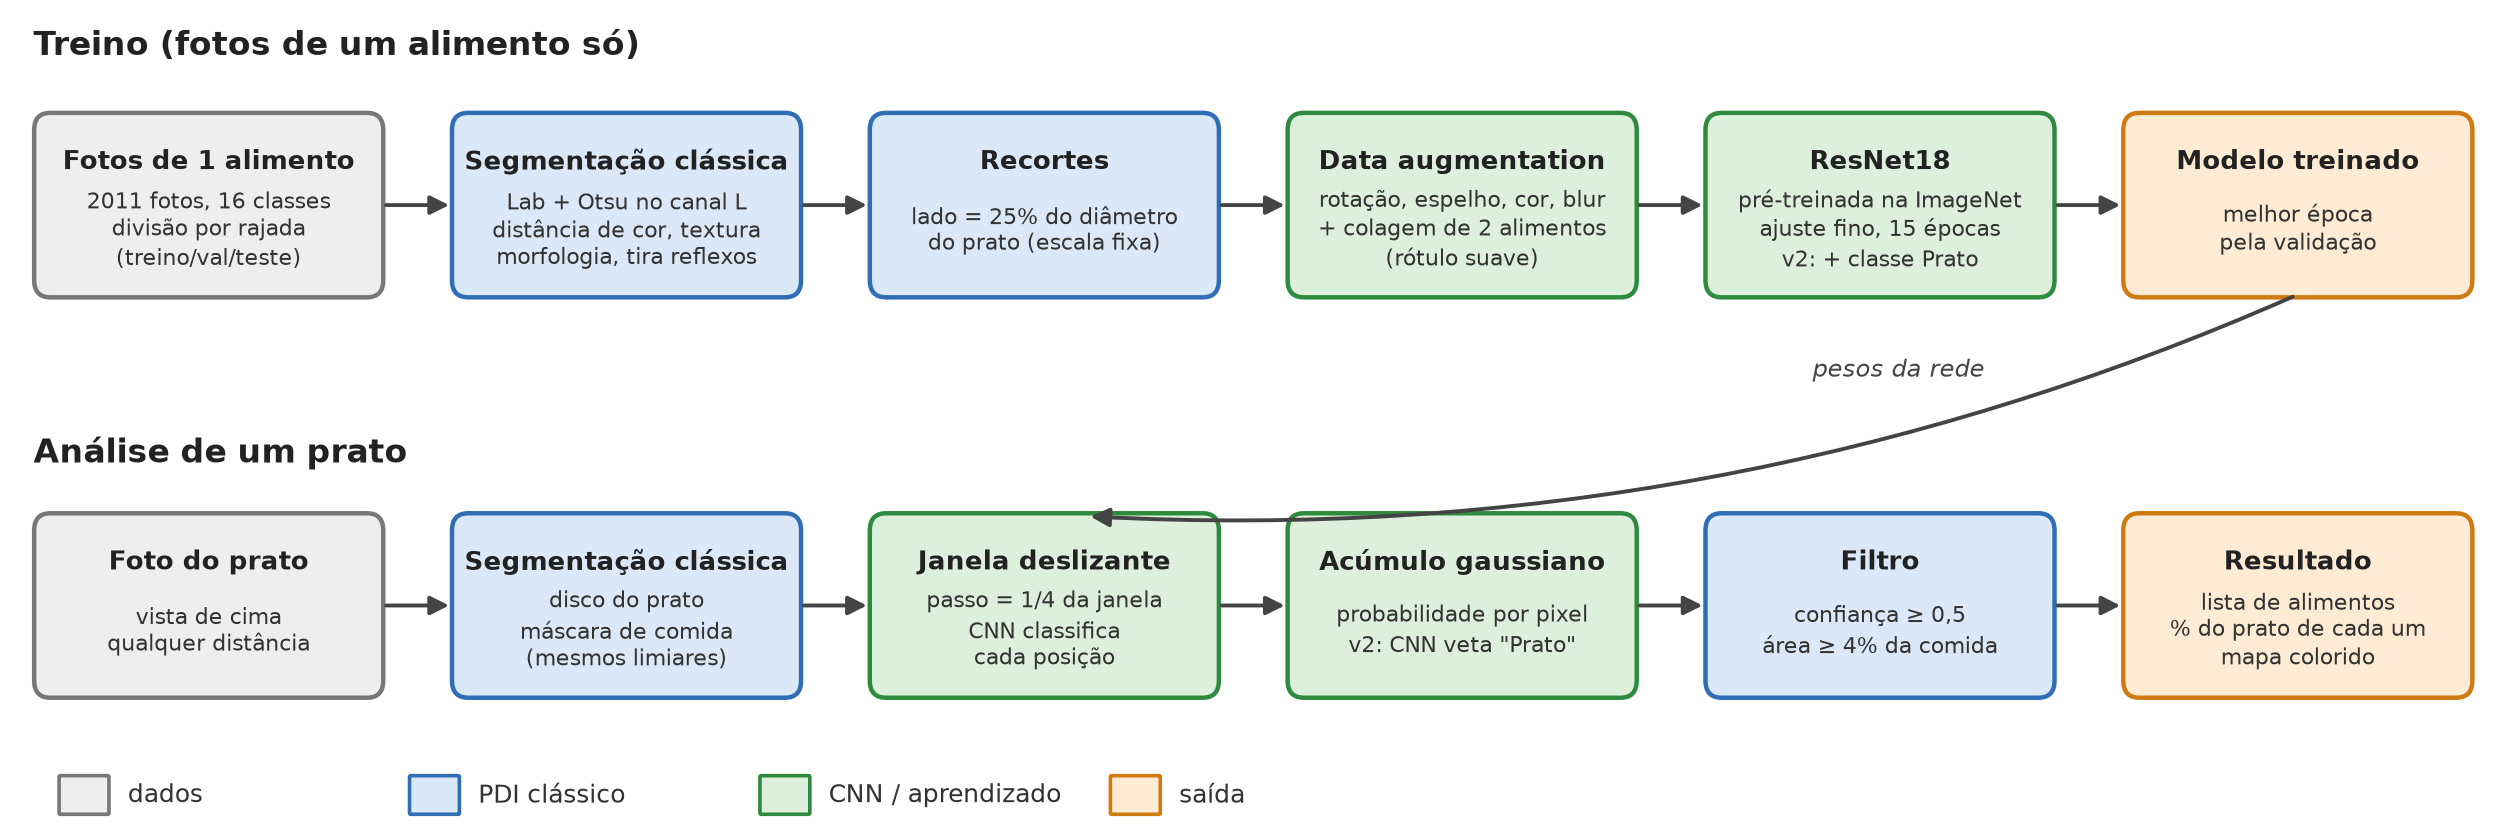
\includegraphics[width=\textwidth]{diagrama_blocos}
	\caption{Diagrama em blocos. Acima, o treino com fotos de um alimento; abaixo, a análise de um prato. Azul: PDI clássico; verde: CNN.}
	\label{fig:blocos}
\end{figure}

\subsection{Dados e segmentação}

O banco tem 2011 fotos de 16 alimentos isolados e 289 fotos de pratos. As fotos foram tiradas em rajadas (várias do mesmo prato, com segundos de diferença); para não vazar fotos quase iguais entre treino e teste, cada rajada foi inteira para um único conjunto: 1093 fotos de treino, 468 de validação e 450 de teste. Os 34 pratos foram rotulados à mão pela autora; alimentos fora das 16 classes (feijão preto, nuggets etc.) foram marcados como OUTRO e não entram nas métricas.

Na segmentação (Figura~\ref{fig:segm}), o prato é o maior componente claro após Otsu no canal $L$, fechado pela envoltória convexa, e a comida é $d > 8$ ou textura $> 3$. Os limiares foram escolhidos por inspeção do arroz, o pior caso (branco sobre branco); com os limiares iniciais (14 e 9) ele não era segmentado. Nas fotos de treino, manchas sem cor e mais claras que o prato (reflexos do flash) são removidas.

\begin{figure}[!htb]
	\centering
	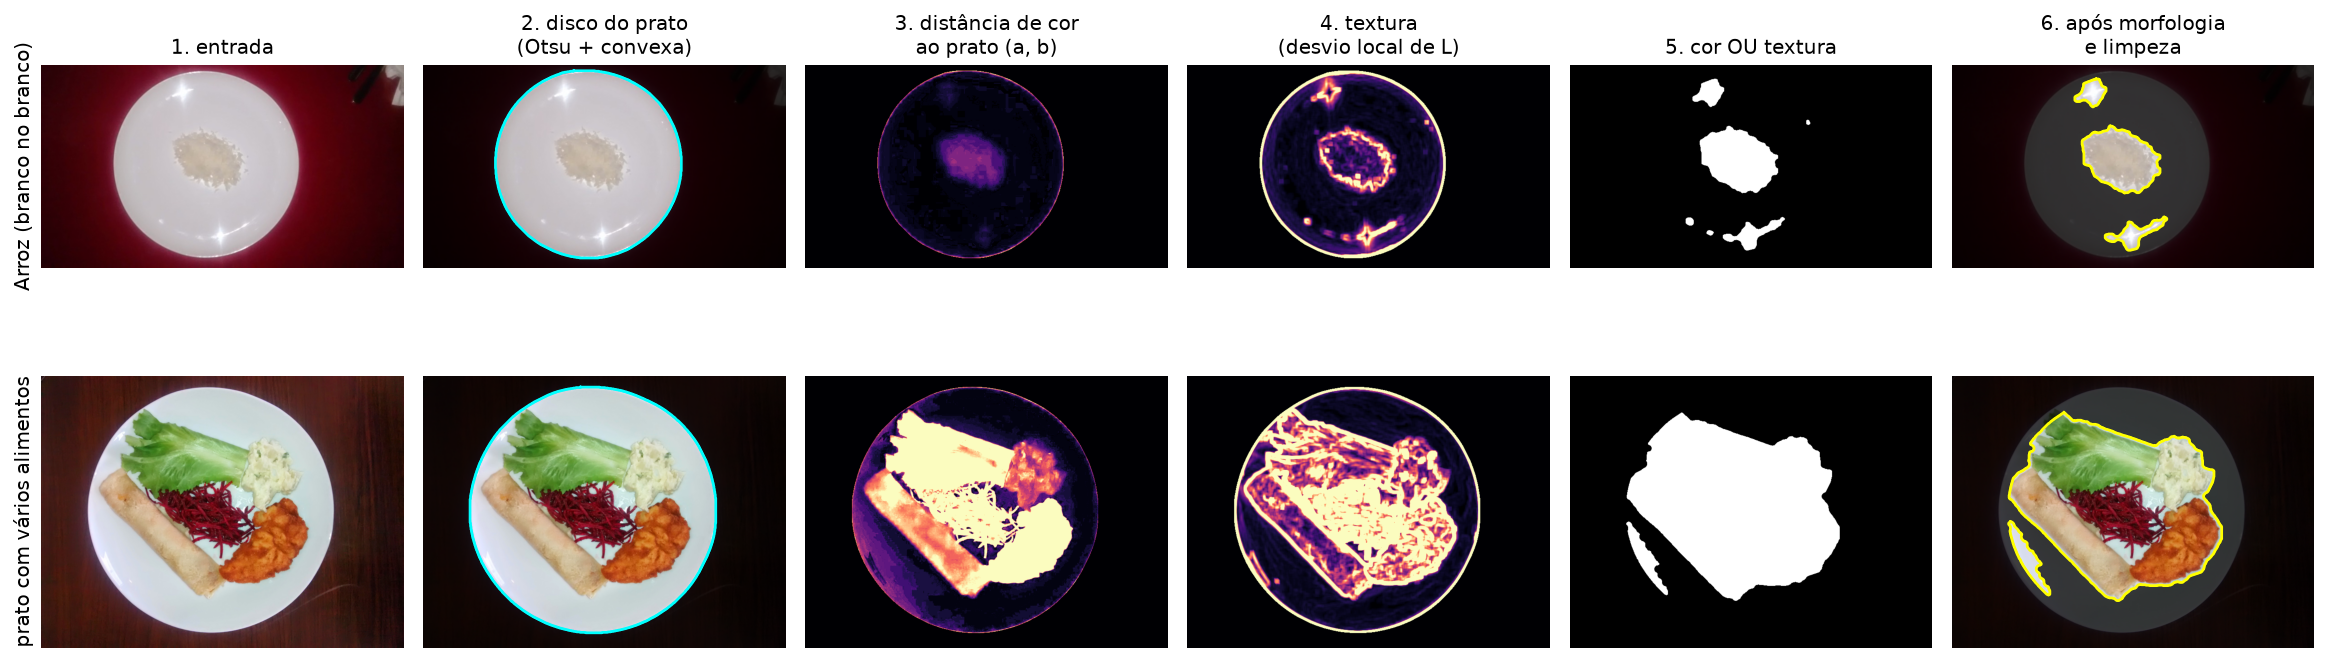
\includegraphics[width=\textwidth]{segmentacao_etapas}
	\caption{Etapas da segmentação clássica para uma foto de arroz (acima) e um prato com vários alimentos (abaixo).}
	\label{fig:segm}
\end{figure}

\subsection{CNN, augmentation e análise do prato}

Uma ResNet18 com pesos pré-treinados da biblioteca torchvision classifica recortes de $160\times160$ pixels cujo lado é 25\% do diâmetro do prato, o que os torna independentes da distância da câmera (AdamW, 15 épocas, melhor época pela validação). Foram comparados três níveis de augmentation: \textit{sem aug} (recortes fixos); \textit{com aug} (posição, tamanho, rotação, espelhamento, cor e desfoque); e \textit{com aug + colagem}, em que 40\% dos recortes juntam dois alimentos separados por uma borda ondulada, com rótulo suave proporcional à comida visível (Figura~\ref{fig:colagem}). A colagem imita alimentos encostados, situação que não existe no treino. A versão v2 acrescenta a classe Prato (prato vazio).

\begin{figure}[!htb]
	\centering
	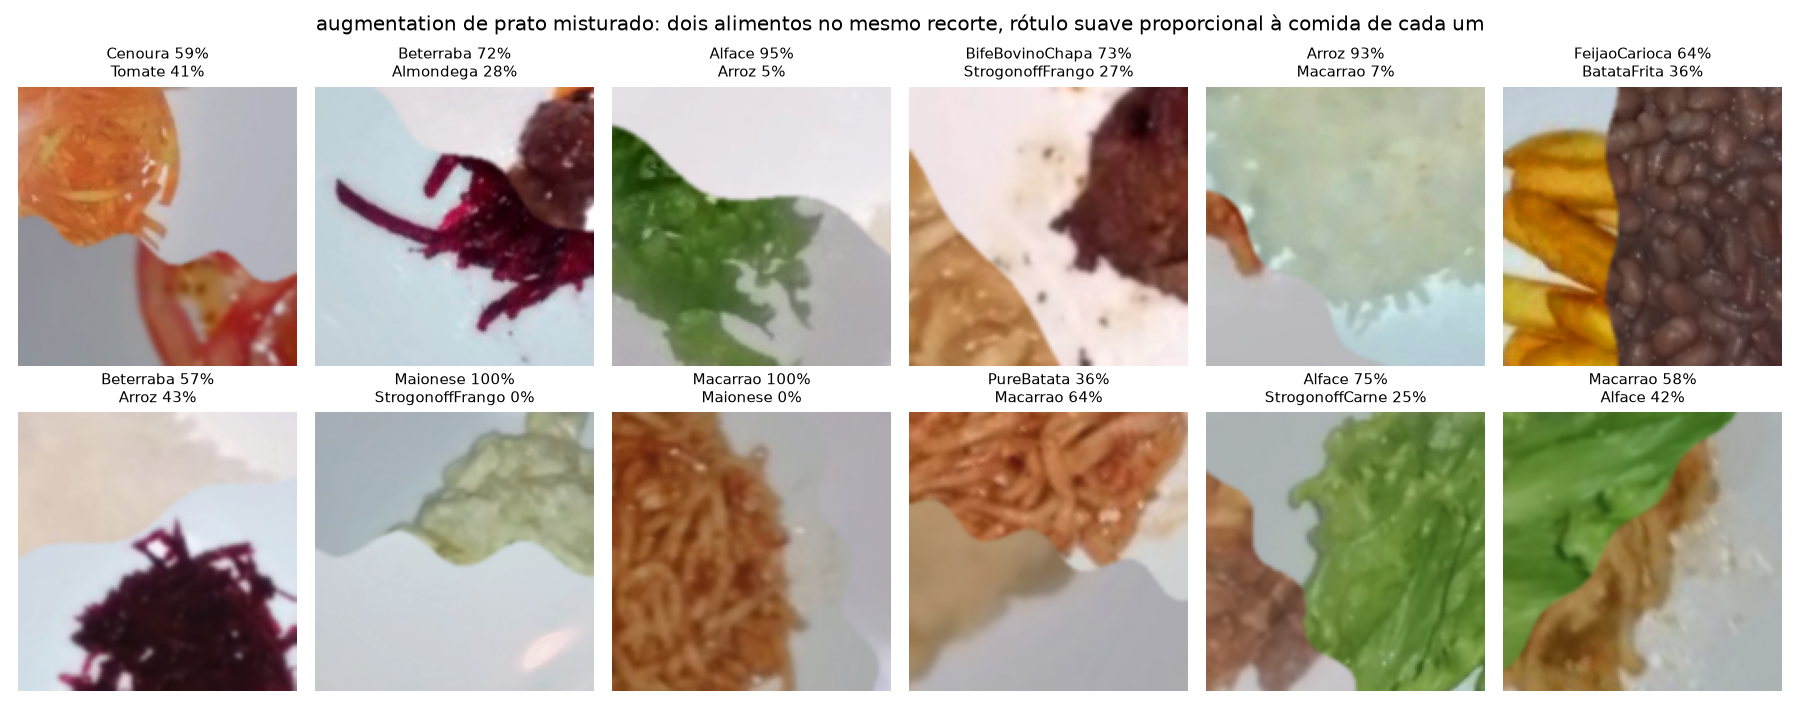
\includegraphics[width=0.68\textwidth]{augmentation_mistura}
	\caption{Augmentation por colagem: dois alimentos no mesmo recorte, com rótulo suave.}
	\label{fig:colagem}
\end{figure}

Para analisar um prato, uma janela percorre a comida com passo de 1/4 da janela, e as probabilidades da CNN são acumuladas nos pixels com peso gaussiano. Um alimento entra na resposta se ocupar ao menos 4\% da comida com confiança acima de 0,5; na v2, a CNN também remove as regiões que reconhece como prato vazio.

Os arquivos entregues contêm o código em Python, a demonstração ao vivo (\texttt{demo.py}), imagens de teste e um \texttt{README.md} com as instruções de instalação e uso.

\section{Resultados e conclusões}

\textbf{Segmentação.} Contra a comida contornada à mão em 20 fotos (10 de alimento isolado, do conjunto de teste, e 10 pratos), a segmentação final quase não perde comida (recall de 0,998), mas marca área a mais (IoU e precisão de 0,73): metade do excesso é uma faixa de até 6 pixels em volta da comida e o restante, caldo no prato. Os limiares iniciais têm IoU médio parecido (0,71), porém falham por completo em alguns casos (arroz com IoU 0). Como comida perdida na segmentação não é recuperada depois, trocar precisão por recall foi a escolha adequada.

\textbf{Alimento isolado.} Todos os modelos acertam 100\% das 450 fotos de teste, exceto a v2 com aug (99,8\%, um purê classificado como maionese). Sem augmentation a perda de treino vai a zero e a validação oscila, sinal de sobreajuste. Os 100\%, porém, escondiam um atalho, revelado pelo Grad-CAM (Figura~\ref{fig:gradcam}): com os limiares iniciais, os recortes de arroz eram pedaços de prato vazio, e a rede aprendeu que ``prato vazio = arroz''. Após a correção dos limiares, a ativação fica sobre os grãos.

\begin{figure}[!htb]
	\centering
	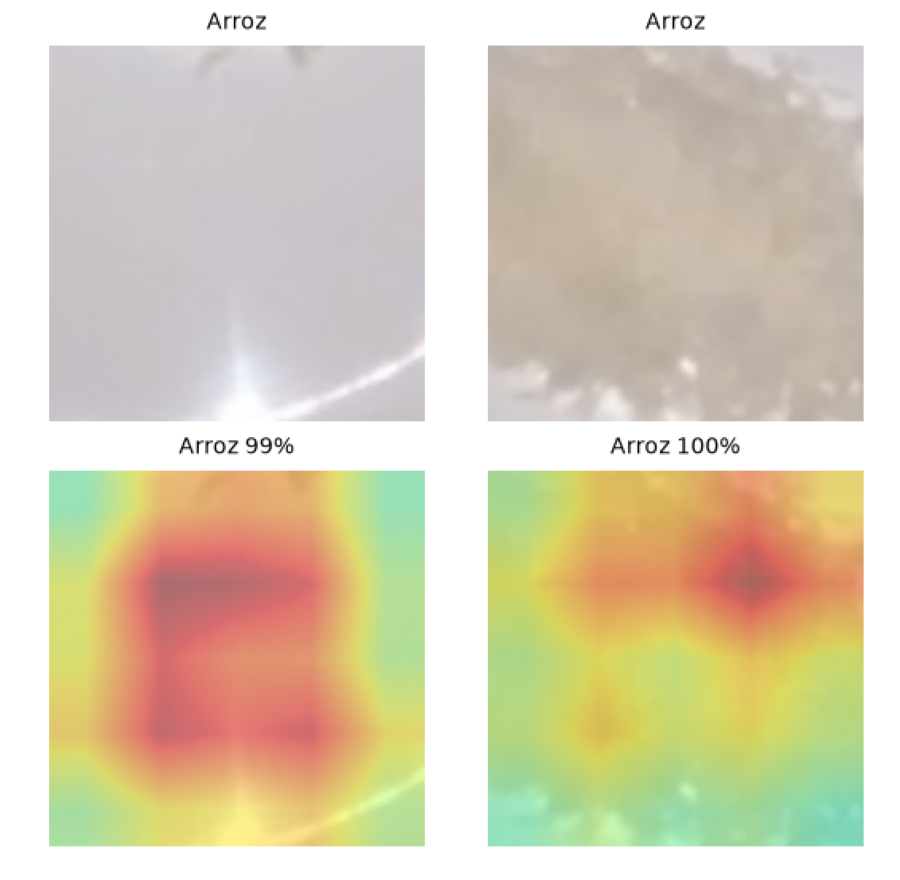
\includegraphics[width=0.34\textwidth]{gradcam_arroz_antes_depois}
	\caption{Grad-CAM da classe Arroz. Esquerda: com os limiares iniciais (14 e 9), o recorte é prato vazio e a rede responde Arroz com 99\%. Direita: com os limiares finais (8 e 3), o recorte contém arroz e a ativação fica sobre os grãos.}
	\label{fig:gradcam}
\end{figure}

\textbf{Pratos.} O F1 cai para 0,84 a 0,88 (Tabela~\ref{tab:pratos}), efeito da mudança de alimentos isolados para misturados. Só trocar a semente aleatória muda o F1 em até 0,04, por isso cada modelo foi treinado 3 vezes. A augmentation genérica deu +0,01 de F1 macro, a favor em apenas 2 de 3 sementes: não se distingue do ruído. A colagem deu +0,024 (v1) e +0,030 (v2) sobre ela, a favor nas 6 comparações com a mesma semente, e recuperou os alimentos claros (na v2, o recall do arroz subiu de 61\% para 87\%), embora o da beterraba tenha caído de 94\% para 77\%. Por prato, a diferença pareada de Jaccard foi de +0,018, com IC 95\% $[-0{,}02;\ +0{,}05]$: consistente entre treinos, mas pequena perto da variação entre 34 pratos. A Figura~\ref{fig:exemplo} mostra o resultado de cada etapa num prato com seis alimentos: a segmentação clássica delimita o prato e a comida, e a janela deslizante atribui um alimento a cada região.

\begin{figure}[!htb]
	\centering
	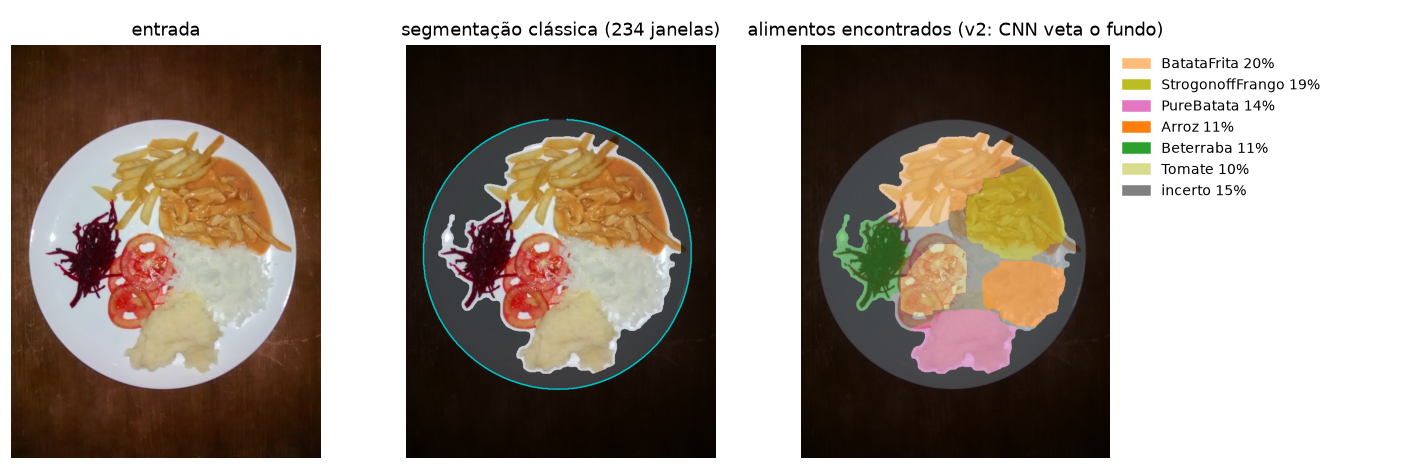
\includegraphics[width=\textwidth]{exemplo_prato}
	\caption{Etapas da análise de um prato com o modelo final (v2 com colagem): foto de entrada, segmentação clássica (contorno do prato em azul e da comida em branco) e alimentos encontrados, com a porcentagem da comida ocupada por cada um. Os seis alimentos foram identificados corretamente.}
	\label{fig:exemplo}
\end{figure}

\begin{table}[!htb]
	\centering
	\caption{Avaliação nos pratos (289 fotos, 34 pratos): média $\pm$ desvio padrão de 3 treinos com sementes diferentes.}
	\label{tab:pratos}
	\small
	\begin{tabular}{lcccc}
		\toprule
		Modelo & F1 macro & F1 micro & Acerto exato & Jaccard \\
		\midrule
		v1 sem aug & 0,836 $\pm$ 0,014 & 0,872 $\pm$ 0,014 & 37 $\pm$ 6\% & 0,80 $\pm$ 0,02 \\
		v1 com aug & 0,844 $\pm$ 0,022 & 0,880 $\pm$ 0,012 & 43 $\pm$ 5\% & 0,81 $\pm$ 0,02 \\
		v1 com aug + colagem & 0,868 $\pm$ 0,013 & 0,905 $\pm$ 0,011 & 47 $\pm$ 6\% & 0,84 $\pm$ 0,02 \\
		\midrule
		v2 sem aug & 0,837 $\pm$ 0,022 & 0,881 $\pm$ 0,015 & 41 $\pm$ 5\% & 0,81 $\pm$ 0,02 \\
		v2 com aug & 0,847 $\pm$ 0,007 & 0,885 $\pm$ 0,004 & 43 $\pm$ 3\% & 0,82 $\pm$ 0,01 \\
		\textbf{v2 com aug + colagem} & \textbf{0,876 $\pm$ 0,005} & \textbf{0,908 $\pm$ 0,002} & \textbf{48 $\pm$ 1\%} & \textbf{0,84 $\pm$ 0,00} \\
		\bottomrule
	\end{tabular}
\end{table}

O principal erro são alimentos fora das 16 classes, sempre trocados por um conhecido (feijão preto vira feijão carioca), pois a softmax não tem opção de rejeição: o Jaccard é 0,88 nos pratos só com alimentos conhecidos e 0,60 nos demais. A classe com pior desempenho é carne bovina de panela, confundida com strogonoff. Ajustar os limiares de decisão por validação cruzada entre pratos não melhorou o resultado, indicando que 34 pratos não bastam para ajustar parâmetros sem sobreajuste.

Em resumo, treinando só com alimentos isolados, o sistema identifica os alimentos de pratos com F1 macro de 0,876 $\pm$ 0,005. A segmentação clássica foi essencial, por fornecer a máscara de comida e a escala do prato. A augmentation desenhada para o problema (colagem) superou a genérica em todas as comparações, e o trabalho mostrou que 100\% de acurácia pode esconder um atalho e que comparar modelos exige várias execuções. As limitações são os rótulos e máscaras feitos por uma única pessoa, o pequeno número de pratos e a falta de rejeição de alimentos desconhecidos. Como melhorias, sugerem-se rotular os pixels de parte dos pratos para treinar uma rede de segmentação semântica, incluir um critério de rejeição, ampliar os pratos de teste e estimar a porção de cada alimento, que é o propósito original do banco.

% Referências Bibliográficas (fonte menor e itens mais juntos pra caber em 5 páginas)
\let\OLDthebibliography\thebibliography
\renewcommand\thebibliography[1]{\OLDthebibliography{#1}\setlength{\parskip}{0pt}\setlength{\itemsep}{1pt plus 0.3ex}}
{\small
\bibliography{bibliografia}
\bibliographystyle{plain}
}

\end{document}
